
\documentclass[a4paper,11pt]{article}

\usepackage[spanish, activeacute]{babel}
\usepackage[ansinew]{inputenc}
\usepackage{graphicx}

\renewcommand{\labelitemii}{\Radioactivity}

%PSUDO

% PSEUDOCODIGO
\newcounter{linea}
\newenvironment{pseudo}{
	\setcounter{linea}{0}
    \begin{small}
    \begin{tt}
    \begin{tabbing}
        ------ \= ---- \= ---- \= ---- \= ---- \= ---- \= ---- \kill
} {
    \end{tabbing}
    \end{tt}
    \end{small}
}

\newcommand{\n}{
    \addtocounter{linea}{1}
    \arabic{linea}.
}

\newcommand{\tab}{\>}
%END PSEUDO
\begin{document}

\markboth{left head}{KANON dbms Technical report } \pagestyle{myheadings} 

\title{
	\mbox{\Huge Base de Datos}\\
	%\mbox{\Huge Trabajo Pr�ctico Final}\\
	\mbox{}\\
	\mbox{\it Implementaci�n de algoritmo de ARIES }\\
	\mbox{\it sobre desarrollo de DBMS}\\
	\mbox{}\\
	Departamento de Computaci�n \\
	Facultad de Ciencias Exactas y Naturales\\
	Universidad de Buenos Aires
\date{}
}
\maketitle
\begin{center}
	\begin{tabular}{cc}
		Luciano Leggieri&Julian Berl�n\\
		{\small \verb"lleggieri@dc.uba.ar"}&{\small \verb"jberlin@dc.uba.ar"}\\
		\cr
		Victor Cabas&Facundo Pippia\\
		{\small \verb"vcabas@dc.uba.ar"}&{\small \verb"facundomensajes@hotmail.com"}\\
	\end{tabular}
	\vskip 5 mm
	Director:\\
	Alejandro Eidelsztein\\
	{\small \verb"ae0n@dc.uba.ar"}\\
\end{center}

{\centering {\bf Abstract}\\}
ARIES es un algoritmo de recuperaci�n muy popular que usa un enfoque steal / no-force. Comparado con otros esquemas de recuperaci�n, es simple y soporta diferentes grados de granularidad en los bloqueos. Luego de una ca�da, este algoritmo procede en tres fases para dejar la base de datos en el estado que tenia antes del crash. El objetivo de este trabajo es realizar una implementaci�n de ARIES en un motor de base de datos construido �ntegramente en Java. 

\vskip 5 mm

\texttt{Keywords: Bases de datos relacionales, ARIES, Transacciones, Recovery Manager}
\newpage
\tableofcontents
\newpage
\listoffigures
\newpage

\newpage

\section{Introducci�n}

\subsection{Objetivos}

El objetivo de este trabajo es construir un motor de base de datos relacional con fines acad�micos, para poder obtener una herramienta que permita una visi�n profunda de \textbf{\textit{c�mo}} funciona un DBMS por dentro. Este proyecto se especializa en mostrar el trabajo de concurrencia transaccional y recuperaci�n del motor. Para la parte de recuperaci�n, este motor se basa en la familia de algoritmos ARIES \cite{ARIES}, el cual posee ciertas propiedades deseables en un m�todo de recuperaci�n eficiente y seguro.\\

Las bases de datos acad�micas existentes, suelen concentrarse en el funcionamiento del analizador sint�ctico, conversi�n a Algebra Relacional de la consulta, y posterior optimizaci�n de la misma. Suelen proveer �ndices basados en �rboles B+, as� como diversos m�todos para la persistencia de tablas en disco y m�todos de paginaci�n en el Buffer Manager.
Sin embargo, temas tan importantes como procesar varias consultas de manera simult�nea y el sistema de recuperaci�n de la base de datos frente a desastres, suelen ser ignorados por estos motores educacionales. Esto conlleva a que los interesados en aprender el funcionamiento de un DBMS, solo obtengan la teor�a en lo que respecta al manejo de transacciones (concurrencia y control de bloqueo de datos) y recuperaci�n de las mismas en caso de una ca�da imprevista del motor.\\


\subsection{Problema a tratar}

Con este proyecto se intenta solventar esta falencia en lo que respecta a motores acad�micos, proveyendo de un motor de base de datos educacional que muestre, tanto en la implementaci�n como en el uso, a aquellos m�dulos encargados del manejo transaccional de las consultas a la base (Transaction Manager, Lock Manager) y recuperaci�n de aquellas que hayan terminado pero sus contenidos no estuvieran volcados en un medio persistente (Recovery Manager).
Este motor tambi�n tiene como finalidad dotar al Departamento de Ciencias de la Computaci�n \cite{DCFCEN} de nuestra facultad \cite{FCEN}, de una herramienta para mostrar y ense�ar el funcionamiento interno de una base de datos relacional con soporte de transacciones y recuperaci�n.\\

En la b�squeda de soluciones similares en distintos departamentos de las universidades del mundo, hemos encontrado que aquellas que muestran el funcionamiento de un DBMS, se concentran, como ya fue mencionado, en el an�lisis y optimizaci�n de consultas. Solo se ha visto un trabajo que extiende a una base de datos educacional existente, agreg�ndole soporte de transacciones y recuperaci�n \cite{MINIREL}.\\

\subsection{Nuestro aporte}

La contribuci�n de este proyecto es la construcci�n de un motor de base de datos con fines educativos. Esto nos dio los objetivos de hacerlo simple, documentar su implementaci�n y que sea posible mostrar, cuando se encuentra en uso, qu� es lo que va haciendo, as� como el estado interno de las estructuras del sistema.\\

Para la construcci�n del motor nos hemos basado en lo aprendido durante la cursada de Bases de Datos \cite{BDFCEN}, y en la bibliograf�a de la c�tedra \cite{RAMA03}, \cite{ULLMAN88} y \cite{BERN87}\\

Como trabajo durante del curso, se nos pidi� que el motor soporte el aborto de transacciones y recuperaci�n de las mismas en caso de ca�das, pero el �nico requisito era que el log de los eventos sea construido utilizando la t�cnica WAL, por lo que se realiz� un sistema simple pero funcional. Luego, como trabajo final, se decidi� cambiar este sistema por uno basado en ARIES, aunque manteniendo el fin educativo y de simplicidad en la implementaci�n.\\

Como se ampliar� posteriormente, ARIES nos ha permitido que el Buffer Manager utilice un esquema STEAL / NO-FORCE \cite{RAMA03}, el cual simplifica la implementaci�n del mismo. Tambi�n era requisito que el sistema de bloqueos se encuentre basado en el algoritmo Two Phase Locking. Hemos extendido este requisito y agregamos soporte para los cuatro niveles est�ndares de aislamiento \cite{SQL92}.\\

El trabajo tambi�n contiene un peque�o sistema de �ndices basados en hash para proveer mayor concurrencia entre consultas paralelas. Estas consultas son escritas en formato SQL est�ndar, y el motor se encarga de analizar y descomponer la sentencia SQL para luego poder ejecutarla sobre la base de datos.\\

Para visualizar el funcionamiento del motor, y proveer una manera de ejecutar consultas y ver sus resultados, se dispone de un cliente gr�fico \cite{KANONOP}, el cual permite simular muchas conexiones al servidor, con fines de poder ejecutar varias sentencias de manera concurrente. Este cliente tambi�n informa del estado de los objetos bloqueados y liberados durante el transcurso de cada transacci�n, y muestra los eventos del log correspondientes a cada operaci�n dentro de las mismas.\\

Para el dise�o del motor nos hemos desviado de los cl�sicos algoritmos procedurales mostrados en los distintos papers, para intentar un acercamiento orientado a objetos. Esto incluye el uso de patrones de dise�o y una arquitectura modular para un mayor entendimiento de cada componente, as� como permitir modificaciones de las mismas por separado sin necesidad de cambiar a las dem�s.\\


\newpage
\section{Estado del arte}

Actualmente hay una inmensa variedad de DBMS tanto con fines industriales como educativos. En esta secci�n se muestran los proyectos y sistemas mas relevantes cuyas implementaciones nos parecieron interesantes sobre todo lo que respecta al tratamiento de transacciones y la recuperaci�n.\\

\subsection{DBMS para prop�sitos acad�micos y de investigaci�n}

Entre los motores de base de datos educativos m�s importantes se encuentran:\\

MINIBASE, es una base de datos de objetivo educacional. Tiene implementados el Buffer Manager, �ndices B+ y Disk Space Manager. No tiene implementada la parte de concurrencia, transacciones y recuperacion del sistema \cite{MINIBAS}.\\

MINIREL es una RDBMS multi-usuario simple que se basa en ARIES para el manejo del log y recuperaci�n.
Implementa la cola del log con una sola p�gina que mantiene en memoria compartida. La lectura y escritura de la misma es mutuamente excluyente.
Tiene limitaciones de baja concurrencia en el Log Manager y asume crash simples provocados por el propio sistema \cite{MINIREL}.\\

LEAP es una base de datos con soporte multiusuario que usa como lenguaje de consultas el �lgebra Relacional (base te�rica para lenguajes como SQL) que maneja tambi�n concurrencia y transacciones \cite{LEAP}.\\ 

System R es una base de datos construida como un proyecto de investigaci�n en el IBM San Jose Research en los a�os '70. Su sistema de recuperaci�n se basa en el protocolo DO-UNDO-REDO, el cual divide a las p�ginas de la base en dos modelos: \textit{nonshadowed} y \textit{shadowed}. En el primero no hay recuperaci�n autom�tica frente a una caida del sistema o el aborto de una transacci�n; en el segundo, se guardan versiones de las p�ginas modificadas por si es necesario restaurarlas a un estado anterior. Mas detalles pueden encontrarse en \cite{GRAY80}.\\

University Ingres, Berkeley Ingres o Ingres89 es la versi�n original de Ingres desarrollada en UC Berkeley durante la d�cada del 70; la primera implementaci�n de un sistema de administraci�n de base de datos relacional.
Usa \textit{QUEL} (QUEry Language) como DML, y el funcionamiento y la confiabilidad son solamente justos a adecuado.
Este sistema multiusuario brinda una vista relacional de datos, soporta dos niveles altos de sublenguajes de datos no procedural, y funciona como una colecci�n de procesos usuario sobre sistema operativo UNIX.
Para la recuperaci�n se utitiza un archivo temporal por proceso, el cual se borrar� o se ejecutar� nuevamente si es que el proceso actual ya hab�a comenzado \cite{STONE76}.

\subsection{DBMS para prop�sitos comerciales}

DERBY es una DBMS comercial y gratuita, implementada en JAVA.
Basa el manejo de log de transacciones y recuperaci�n en los algoritmos de ARIES.
Tiene algunas diferencias con el est�ndar ARIES:\\

\begin{itemize}
	\item En vez de guardar el pageLSN con la p�gina, guarda un n�mero de versi�n de la misma.
\end{itemize}


\begin{itemize}
	\item No guarda una tabla de p�ginas sucias en el checkpoint. Durante el checkpoint solamente fuerza las paginas a disco.
\end{itemize}

 
\begin{itemize}
	\item El Undo empieza en el LSN actual al momento de comenzar el checkpoint.
\end{itemize}

\begin{itemize}
	\item En en el reinicio del motor, Derby hace el Redo o el Undo seg�n el que tenga LSN mas chico para empezar.
\end{itemize}

\begin{itemize}
	\item 	Usa transacciones internas en vez de Nested Top Level Actions para separar los cambios 	  					estructurales de las operaciones normales.
\end{itemize}

\begin{itemize}
	\item Derby omite la fase de an�lisis en el reinicio del motor ya que no lo requiere por la forma 					en la que hace los checkpoints.
\end{itemize}

Mas informaci�n sobre Derby en \cite{DERBY}\\

ALTIBASE es un motor de base de datos relacional de alta performance y tolerancia a fallas que maximiza el uso de la memoria principal para las operaciones logrando una gran performance. Est� pensada principalmente para dispositivos m�viles.
Un Log Flush Thread se encarga de enviar el log a disco sin interferir con las transacciones activas.
El log se escribe en m�ltiples archivos para mejorar eficiencia en la recuperaci�n.
Tambi�n separa las transacciones en distintos niveles de durabilidad, usa un buffer de memoria y otro archivo de mapeo a memoria, ambos como buffer de log.
En los niveles m�s altos, un thread sincroniza con un archivo de log en disco.
En los niveles m�s bajos, no garantiza la durabilidad del commit ya que en �stos el estado de commit de la transacci�n se pone antes de ser escrito en el archivo de log.
Tambien provee distintos niveles de logging bas�ndose en la importancia entre la performance de la transacci�n y la consistencia  de los datos \cite{ALTIBAS}.\\

SQL Server tambien usa ARIES en su Recovery Manager, junto con el protocolo WAL. Para que una transacci�n asegure su estado de commit todos sus registros de log deben estar escritos en disco.
Tiene un enfoque NO FORCE. Soporta locking a nivel registro, rango, p�gina o tabla.
La tasa de transacciones se incrementa usando transacciones peque�as \cite{KB230785}.\\

Tanto \cite{ARIES} como \cite{ARIESRH} mencionan la implementaci�n de los algoritmos ARIES en la familia de productos DB2 de IBM.\\
DB2 guarda im�genes del espacio de tablas y va a la �ltima estable que ten�a (en vez de tener que ir al primer registro de log y rehacer toda la operaci�n). DB2 usa entradas en la tabla SYSCOPY para identificar y localizar la copia m�s reciente a tomar para restaurar. Entonces aplica los cambios a los datos siguiendo la secuencia del log. QUIESCE utility es una utilidad para establecer un punto de consistencia para un table space o un conjunto de table spaces logicamente relacionados. REPORT RECOVERY recopila info de SYSIBM.SYSCOPY y SYSIBM.SYSLGRNX (que son parte del directorio de DB2) para brindar informaci�n importante para la recuperaci�n. Hay dos tipos de metodos de recovery: \textit{to current (al m�s reciente punto de consistencia)} es el est�ndar para errores de hardware o software; \textit{to a specific point-in-time (a un punto espec�fico)} se aplica mayormente a errores de aplicaci�n \cite{BRUNI02}.\\


Oracle es uno de los motores de base de datos relacionales mas importantes de la industria y  
es usado a gran escala por muchas compa��as y multinacionales.
Para su recovery manager (RMAN) utiliza una tecnolog�a llamada \textit{Flashback}, la cual  
consiste en un conjunto de m�todos para recuperar la integridad de la base de datos luego de  
producido un crash o un error humano.
Entre las caracter�sticas mas importantes que brinda la tecnolog�a Flashback se encuentra la  
posibilidad de generar consultas a versiones antiguas del esquema de objetos, generar  
consultas de la informaci�n hist�rica de la base de datos y realizar un auto-reparaci�n de  
informaci�n l�gica corrupta; todo esto mientras la base de datos se encuentra online.
Por otro lado no hay mucha informaci�n disponible acerca de qu� m�todos y enfoques utiliza  
Oracle en su Recovery Manager \cite{ORACLE}.\\





 


\newpage

\section{Dise�o} 
\subsection{Modelo propuesto}

El sistema sigue el protocolo Cliente - Servidor, donde toda la complejidad del motor de base de datos se encuentra en el servidor. El cliente es una aplicaci�n liviana encargada de la comunicaci�n con el usuario, enviando los pedidos de consultas al servidor, esperando por el resultado y mostrando al mismo por pantalla.\\

\begin{figure}[h]
		\centering
		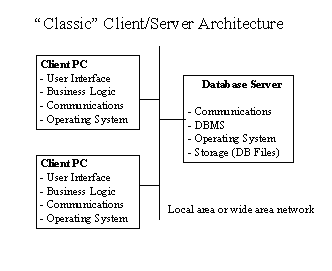
\includegraphics[scale=0.8]{img/ClienteServerArchitecture.png}
		\label{fig:ClienteServerArchitecture.png}
		\caption{Arquitectura del modelo Cliente / Servidor}
\end{figure}



Este modelo permite una mejor abstracci�n y separaci�n de la funcionalidad propia del motor, con aquella encargada de la interfaz al mundo exterior. Siguiendo un esquema de env�o de mensajes, ambos programas pueden ejecutarse tanto en la misma m�quina como en computadoras distintas, sin perder ninguna clase de utilidad.\\

\subsection{Arquitectura del servidor}

Teniendo en cuenta los fines acad�micos del trabajo, se decidi� separar cada componente del servidor en m�dulos bien diferenciados e independientes, tratando de maximizar la cohesi�n y tener un bajo acoplamiento. Cada modulo respeta una interfaz, la cual es usada por aquellos que lo acceden, deslig�ndose as� de c�mo est� implementado cada uno.
Esto permite poder modificar a futuro la implementaci�n de un modulo sin que ello afecte a los restantes, mientras se respeten las interfaces establecidas en el sistema.
El enfoque esta basado en un dise�o orientado a objetos, haciendo uso de diferentes patrones de dise�o para poder facilitar el entendimiento de cada modulo y proveer de soluciones est�ndar. Cada objeto tiene un prop�sito espec�fico y diferenciable, lo que permite un mayor entendimiento del desarrollo de los m�dulos y funcionamiento del motor.\\

En la figura 2 muestran los m�dulos e interrelaciones existentes en el sistema:\\

\begin{figure}[h]
		\centering
		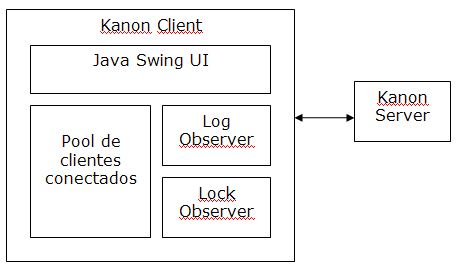
\includegraphics[scale=0.6]{img/arquitectura.png}
		\label{fig:arquitectura.png}
		\caption{Arquitectura del Servidor Kanon}
\end{figure}

A continuaci�n se explican con mayor detalle aquellas componentes que tienen mayor relevancia con el objetivo de este trabajo. En cada una se puntualiza la trascendencia que tienen los algoritmos de ARIES sobre la misma, enfocando su funcionalidad principal en la secci�n del Recovery Manager.\\


\subsection{Disk Space Manager}

El DiskSpace Manager es el encargado de guardar las p�ginas en un medio de almacenamiento persistente, en nuestro caso mediante archivos en disco duro dentro de un directorio ya preestablecido.\\ 

Las p�ginas se guardan en formato binario. La elecci�n del mismo se debe a:\\

\begin{itemize}
	\item La necesidad de implementar �ndices, o sea que las p�ginas no s�lo contienen informaci�n de las tablas.
\end{itemize}


\begin{itemize}
	\item Por ARIES, ya que en principio, el algoritmo guarda en los eventos de log aquellos cambios de los registros de las tablas a nivel de bytes.
\end{itemize}


\begin{itemize}
	\item Por similitud a un motor de base de datos real.
\end{itemize}

El formato utilizado en un principio hab�a sido XML, y estaba justificado por el hecho de tener un formato m�s legible sin necesidad de transformaci�n alguna. Esto es, se pod�a abrir una p�gina, con cualquier visor de texto, y saber c�mo era su contenido; �til para fines acad�micos. El formato XML tambi�n fue usado en el log de eventos para la recuperaci�n del sistema, el cual fue cambiado por el log de ARIES.\\

Tambi�n hay que destacar que al no realizar la conversi�n XML, el Disk Manager toma una l�gica mucho m�s simple, pues s�lo debe estampar el arreglo de bytes representantes de una p�gina provistos por el Buffer Manager en un archivo en disco. Y viceversa para la lectura.\\

Este manager se completa con m�todos de creaci�n y borrado de p�gina:

\begin{itemize}
	\item Crear de una nueva p�gina. A partir de las p�ginas existentes se obtiene cu�l ser� el n�mero de la nueva p�gina. La implementaci�n est� optimizada para tablas que no necesitan ning�n orden en particular sobre sus registros.
\end{itemize}
 
\begin{itemize}
	\item Borrar una p�gina. Borra el archivo de la p�gina del disco persistente.
\end{itemize}



\subsection{Buffer Manager}

Para el manejo de las p�ginas en el Buffer Manager se utiliza el esquema \textbf{steal / no-force}. Con \textbf{no-force}, al no requerir que la p�gina se guarde en disco estable para cada commit, esta escritura se puede realizar una vez luego que todas las transacciones hayan modificado la p�gina, reduciendo considerablemente la cantidad de E/S. Esta mejora se combina con el enfoque \textbf{steal}, el cual permite que una p�gina que haya sido modificada por una transacci�n en curso, sea guardada en disco y eliminada de la memoria (para hacer lugar a otra p�gina), aumentando la capacidad de la memoria virtual del motor. Luego si esos cambios deben ser deshechos, entrar� en juego el proceso de rollback propuesto por ARIES, leyendo el archivo de log para revertir las modificaciones.\\

Otra posibilidad m�s simple de implementar es el esquema \textbf{no-steal / force}, pero el mismo posee determinadas desventajas. \textbf{No-steal }asume que todas las p�ginas modificadas por las transacciones en curso pueden estar fijas en el pool de p�ginas del Buffer Manager lo cual es una asunci�n no realista, pues limita la cantidad de transacciones que se pueden estar ejecutando de manera concurrente y el tama�o de las mismas. Con \textbf{force}, si una misma p�gina es modificada por muchas transacciones seguidas, �sta se escribe en disco a medida que las transacciones van haciendo commit.\\


\begin{figure}[h]
		\centering
		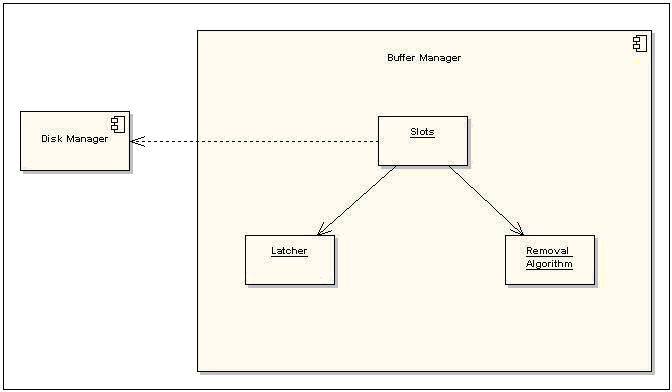
\includegraphics[scale=0.4]{img/BufferManagerDiseno.png}
		\label{fig:BufferManagerDiseno.png}
		\caption{Arquitectura del Buffer Manager de Kanon}
\end{figure}

Otro punto importante tratado por ARIES es el control de acceso a las p�ginas. Las p�ginas disponen de tres tipos de bloqueos:\\

\begin{itemize}
	\item \textbf{pin}:
Sirve para que el algoritmo de remoci�n utilizado por el Buffer Manager no deseche una p�gina que est� siendo usada por una o varias transacciones. Cuando una transacci�n necesita utilizar una p�gina, la fija en el slot. En este trabajo, el manejo de pines corre por parte del subm�dulo Pin Manager. Para cada p�gina un contador indica por cu�ntas transacciones est� siendo usada. Se incrementa al acceder y se decrementa cuando es liberada.

\item \textbf{latch}:
Sirve para insertar un nuevo registro y para que el RecLSN se mantenga ordenado con respecto a las operaciones sobre la p�gina. Esa variable apunta al �ltimo evento del log de ARIES que realiz� una modificaci�n en la p�gina. Tambi�n, por simplicidad, va a estar representado por un Latch Manager propio.
Se obtiene un latch al modificar la p�gina (insert, update o delete), y se libera luego de escribir la entrada del evento en el log de ARIES. No se obtiene ning�n latch al leer.

\item \textbf{lock}:
	Bloqueo est�ndar de p�ginas hecho por el Lock Manager principal. Puede ser utilizado para 				optimizaciones (si una transacci�n tiene bloqueados una gran porcentaje de registros pertenecientes a una misma p�gina, le conviene bloquear toda la p�gina).
En este trabajo este tipo de bloqueo no va a ser realizado.

\end{itemize}
 

La documentaci�n de ARIES muestra los pasos a seguir para evitar deadlock entre lock de registros y latch de p�ginas (esto aplica tambi�n a las p�ginas de los �ndices):\\

\begin{enumerate}

	\item \textbf{update / delete}:
Se bloquea el registro de manera exclusiva y luego se obtiene un latch la p�gina. Si alguien ya tenia el latch de esa p�gina, por el funcionamiento del algoritmo, se sabe que no va a pedir el lock de alg�n registro bloqueado antes de liberar tal latch. 

\item \textbf{insert}:
Se obtiene un latch de la p�gina y se obtiene el ID del nuevo registro. Entonces, se procede a bloquear el ID de manera exclusiva para insertar el registro. Este bloqueo es CONDICIONAL. Si falla, se libera el latch y se intenta bloquear el ID de manera exclusiva INCONDICIONAL. Una vez que se obtenga ese lock, se pide de nuevo un latch de la p�gina y se verifica que ese ID no haya sido usado (justo antes de bloquearlo INCONDICIONAL). Si fue usado, se libera el lock de tal ID y se vuelve repetir toda la operaci�n.

\end{enumerate}

Cuando se desea acceder o modificar una tabla, se le pide al Buffer Manager que traiga las p�ginas correspondientes a memoria, en caso de no encontrase all� con anterioridad. Estas p�ginas ser�n marcadas mientras se est� operando con ellas y luego se liberar�n para que sean removidas en caso de necesitar m�s memoria.\\

El Buffer Manager contiene m�todos para obtener una p�gina, liberarla, crearla, borrarla, saber si se encuentra en memoria y guardar las p�ginas que fueron modificadas. Para la mayor�a de ellos, luego de realizar las acciones necesarias se llama al Disk Space Manager para que persista los resultados.\\
 

\subsection{Ejecutor}

El Ejecutor tiene como objetivo, llamar al analizador para descomponer la sentencia SQL en partes m�s f�ciles de procesar; luego realizar la ejecuci�n y devolver el resultado de la consulta propiamente dicha. Esto se realiza desde el Servidor, quien obtiene las sentencias que son ejecutadas por el cliente.\\

El hecho de existir manejo de �ndices, hace que la ejecuci�n de cl�usulas WHERE (tanto en el select, update como delete) intente acceder por ellos. En el caso de no ser posible, entonces reci�n ah� se procede a recorrer toda la tabla.\\
 
Por simplicidad, no se contemplan joins (no se realiza producto cartesiano).\\ 

Las sentencias que soporta la aplicaci�n son las siguientes:\\

\texttt{
\begin{flushleft}
       INSERT INTO tabla (col1, col2...) VALUES (valor1, valor2...);\\
       INSERT INTO tabla (col1, col2...) SELECT...;\\
       UPDATE tabla SET col1 = expresion WHERE expresionWhere;\\
       SELECT col1, expresion1... FROM tabla WHERE expresionWhere;\\
       DELETE FROM tabla WHERE expresionWhere;\\
       CREATE TABLE tabla (col1 NUMERIC/CHAR(XX)...);\\
       DROP TABLE tabla;\\
       BEGIN TRANSACTION;\\
       COMMIT TRANSACTION;\\
       SAVEPOINT nombre;\\
       ROLLBACK nombre;\\
       ROLLBACK TRANSACTION;\\
       CRASH;\\
       CHECKPOINT;\\
       ISOLATION nivelAislamiento;\\
\end{flushleft}
}

El nivel de aislamiento puede ser Read Uncommited, Read Commited, Repeatable Read y Serializable. M�s informaci�n sobre los mismos aparece en la secci�n correspondiente al Lock Manager.\\


\subsection{Recovery Manager}

El Recovery Manager es el modulo encargado de proveer robustez a una base de datos. Su funci�n consiste en darle las propiedades de atomicidad y durabilidad a las transacciones del motor \cite{RAMA03}.\\ 

Entre las t�cnicas disponibles para realizar este cometido, las m�s conocidas son Shadow Paging \cite{SHAWIK}, \cite{RAMA03} y Write Ahead Logging \cite{WALWIK}, \cite{RAMA03}. Uno de los objetivos de este trabajo es mostrar el funcionamiento de un sistema de recuperaci�n basado en los algoritmos de ARIES \cite{ARIES}. Estos utilizan una estrategia WAL, la cual es menos costosa en t�rminos de memoria.

\begin{figure}[h]
		\centering
		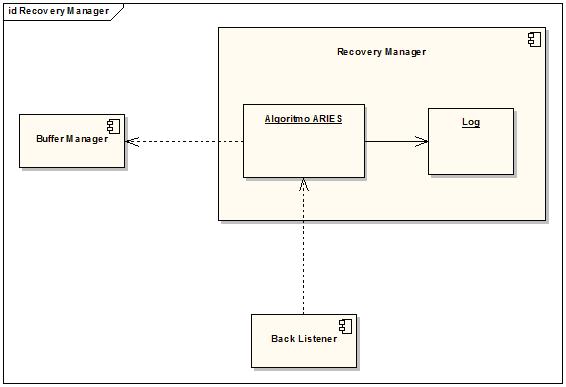
\includegraphics[scale=0.6]{img/RecoveryManagerDiseno.png}
		\label{fig:RecoveryManagerDiseno.png}
		\caption{Arquitectura del Recovery Manager de Kanon}
\end{figure}

Cada evento que ocurre en la base de datos, se guarda en un log, indicando qu� evento es y par�metros asociados al mismo para poder rehacer dicha operaci�n o deshacerla en caso de ser necesario. El archivo de log es de formato creciente, y debe ser guardado en medio persistente cada vez que una transacci�n hace commit, o cuando se realiza un checkpoint de la base de datos \cite{RAMA03}.\\

Cuando se modifica una p�gina, ya sea de una tabla o de un �ndice, el est�ndar de ARIES recomienda que se guarde un evento indicando qu� p�gina fue modificada y cu�les bytes cambiaron dentro de la misma. Teniendo en cuenta los fines acad�micos de este proyecto, se decidi� separar la operaci�n de modificaci�n en valores m�s l�gicos. Se indica si se trata de la inserci�n de un registro, modificaci�n o borrado del mismo, y de la misma manera para los registros de los �ndices.  Esto permite conocer mejor el funcionamiento del motor, ya que una operaci�n de inserci�n se ver� reflejada en el log con un evento de inserci�n, junto al identificador del nuevo registro y los valores correspondientes a cada columna de la tabla afectada (y el agregado de los registros correspondientes a cada �ndice asociado).\\

Siguiendo las referencias de ARIES, cada evento tiene un identificador propio, el cual es basado en su posici�n dentro del archivo de log. Luego, cada transacci�n toma nota del �ltimo evento realizado, y cada p�gina sabe el identificador del �ltimo evento que realiz� una modificaci�n sobre la misma. Cuando una transacci�n realiza commit se toma de este hecho con un evento de commit, y cuando termina (ya sea por commit o un aborto), se marca una finalizaci�n de �sta en el log. Cuando se realiza un aborto de una transacci�n, se deshacen los cambios hechos en orden inverso, y los eventos CLR toman de esto, por si luego hay que volver a deshacer esos cambios.\\

Cuando ocurre una falla y se cae el sistema, al volver a iniciarse, es necesario que aquellas modificaciones que no fueron guardadas de manera persistente sean rehechas, para que no se pierdan estos cambios. Tambi�n es necesario que las transacciones que se encontraban en curso durante la ca�da y no hicieron commit deshagan sus cambios, para que parezca como si nunca hubieran existido. 
Para esto ARIES propone que la recuperaci�n se divida en tres fases: ANALISIS, UNDO y REDO y explica los pasos a seguir en cada fase. Este modulo realiza la recuperaci�n de la misma manera, y se detalla cuando ocurre cada paso. Sin embargo, se decidi� desviarse de la implementaci�n procedural propuesta, por una orientada a objetos.\\

Para asegurarse que los cambios hechos por las transacciones est�n en una memoria persistente, existe el concepto de Checkpoint. �ste fuerza la escritura del log a disco as� como de aquellas p�ginas modificadas desde la �ltima vez que fueron escritas. Las bases de datos suelen tomar un Checkpoint de manera peri�dica. Pero para este motor se decidi� no hacer eso, para poder ver el funcionamiento del sistema de recuperaci�n en caso de una falla. Sin embargo, si se agreg� la funcionalidad de poder realizar un Checkpoint de manera manual, y tambi�n de poder forzar una ca�da del sistema de manera manual (ambas con sentencias SQL propias de esta base de datos).\\

De la misma manera que en los dem�s m�dulos, se agreg� el soporte para savepoints y transacciones anidadas. Las modificaciones para soportar a esta �ltima se realizaron seg�n los algoritmos de ARIES/NT \cite{ARIESNT}. Como los savepoints son entidades l�gicas de una transacci�n, no fue necesario ning�n cambio al sistema de recuperaci�n para soportarlos.\\

Hay eventos que pueden ocurrir dentro de una transacci�n para los que es deseable que no se deshagan, aunque la misma sea abortada. Para realizar esto se implementaron las Nested Top Actions \cite{ARIES} cuya funcionalidad es justamente �sta y en ARIES se explica qu� cambios hay que cometer para soportarlas.\\




\subsection{Transaction Manager}

Este modulo tiene la finalidad de administrar la ejecuci�n de todas las transacciones en curso. 
Tiene una estructura la cual almacena todas las transacciones que se est�n corriendo sobre el Server. Para un cliente dado se puede ver si actualmente tiene una transacci�n en curso. Ya que por cada cliente, se va a tener una thread del servidor ejecutando sus operaciones. Las operaciones de la transacci�n de un cliente no interfieren con las transacciones de los otros clientes.\\

Una transacci�n corresponde a un thread, �stas no pueden ser suspendidas y resumidas en otro thread.\\

El servidor ejecuta concurrentemente transacciones de cada conexi�n con un cliente. Cada conexi�n se asocia a un thread del servidor y para cada uno de estos threads puede haber una transacci�n en curso o ninguna.\\

Para cada sentencia (l�nea de comando que env�a el cliente) se sabe si esta debe ser corrida dentro de una transacci�n o no. Por ejemplo, las instrucciones DML deben serlo, pero para la instrucci�n que realiza un checkpoint no es necesario. Luego, aquellas que lo necesiten van a ser tratadas por el ejecutor como una transacci�n propia si no exist�a ninguna en curso.\\

Se tom� esta decisi�n para que en casos donde una instrucci�n simple trabaje sobre un conjunto de datos, efect�e todas sus acciones o ninguna.Por ejemplo al hacer un update con un set, se van a modificar todos los registros en cuesti�n o ninguno.\\

Lo que hace el ejecutor es fijarse si hay una transacci�n en curso, cuando recibi� la sentencia, si no la hay la crea ( a lo que llamamos Transacci�n Autom�tica) , ejecuta la sentencia y luego se fija en un flag si la transacci�n donde ejecuto la instrucci�n es autom�tica o no, si lo es tiene que finalizarla.

Es posible crear transacciones explicitas del cliente cuando se env�e un Begin Transaction, seguido por una serie de sentencias y finalizando con un Commit o Rollback, y tambi�n se tendr�n transacciones impl�citas cuando el cliente env�e comandos simples como Insert � el ejecutor se va a encargar de ejecutar esta sentencia como Begin Transaction, luego Insert ... y finalizara con un Commit (o un Rollback en caso de haberse lanzado alguna excepci�n).\\

Las transacciones tienen un n�mero como identificador, el cual va siendo incrementado at�micamente. Adem�s, al inicio del sistema, se verifica el log para empezar con el siguiente valor al numero mas alto de las transacciones del log para que los eventos de las nuevas transacciones no se confundan con las ya grabadas.\\

Las propiedades ACID de las transacciones se obtienen de la siguiente manera:\\

\begin{itemize}
	\item Atomicidad: Cuando ocurre un error o se desea abortar la transacci�n, el Recovery Manager basado en ARIES, a trav�s de su log, se encarga de realizar el rollback y restaurar las modificaciones hechas por cada sentencia dentro de la transacci�n a su estado anterior.\\

	\item Consistencia: Como se comenta en \cite{RAMA03} en la secci�n 18.1.1, los usuarios del sistema son responsables de mantener la consistencia de las bases de datos afectadas. Este motor no soporta restricciones de integridad, como claves primarias (o unicidad en los valores de las columnas) y claves for�neas.\\

	\item Aislamiento: El Lock Manager se encarga de las garant�as de serializaci�n de las transacciones que se ejecutan de manera concurrente, y tambi�n se encarga de los bloqueos para aquellas que desean acceder o modificar objetos (registros, tablas) al mismo tiempo.\\

	\item Durabilidad: As� como con la atomicidad, el Recovery Manager se encarga de la recuperaci�n de las transacciones activas al momento de ocurrir una ca�da del sistema. Tambi�n se encarga de rehacer las acciones de aquellas transacciones cuyos cambios no fueron guardados en un almacenamiento no vol�til.\\
\end{itemize}

En la secci�n del Lock Manager se comenta sobre el interlineado de transacciones y el Schedule formado por las mismas.\\

En vistas de dar una mayor profundidad a los temas de transacciones, se han agregado dos extensiones de ARIES para proveer de mayor funcionalidad a este motor, sin dejar de lado los fines educacionales del mismo:\\

\subsubsection{Transacciones anidadas}
En \cite{ARIESNT} se comenta como dar soporte de transacciones anidadas a un sistema de recuperaci�n basado en ARIES, indicando los cambios en el sistema de log y en las tablas de transacciones, se decidi� realizar tales cambios en este motor acad�mico para que futuros interesados puedan conocer funciones avanzadas de una base de datos concurrente. Los cambios en el Transaction Manager implican que para cada thread, no existe una referencia a una transacci�n, sino una lista de transacciones, la lista se encuentra ordenada de la transacci�n de mas alto nivel a aquella mas reciente y profunda en el anidamiento.\\

Cuando se crea una transacci�n anidada, �sta hereda el nivel de aislamiento de la transacci�n padre (y claro est�, se ejecutan en el mismo thread).\\

El m�todo de abortar la transacci�n fue reemplazado por dos m�todos, uno aborta la �ltima transacci�n (La m�s anidada), volviendo a la transacci�n padre, y el otro aborta todas las transacciones del thread. El m�todo de commit realiza la operaci�n solo para la transacci�n mas anidada, y luego el log se encarga de unir esa operaci�n de commit con la transacci�n padre, por si esta luego realiza un rollback. A la transacci�n padre se le actualiza su �ltimo LSN con esta operaci�n de commit de la hija.\\

En las secciones del Lock Manager y Recovery Manager se comentan los cambios hechos para que ambos soporten transacciones anidadas.\\



\begin{figure}[h]
		\centering
		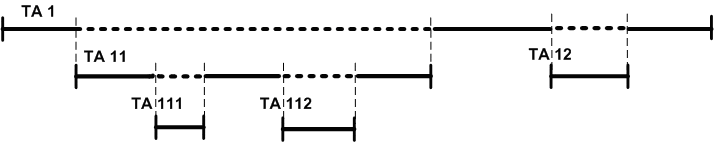
\includegraphics[scale=0.4]{img/TrxAnidadas.png}
		\label{fig:TrxAnidadas.png}
		\caption{Transacciones anidadas seg�n el tiempo de ejecuci�n}
\end{figure}

Cabe destacar que cuando se crea una transacci�n hija, la transacci�n padre es suspendida, pues todas las sentencias nuevas del thread corresponder�n a la transacci�n hija hasta que esta aborte o haga commit. Luego, no es necesario ocultar los cambios de la transacci�n hija al padre pues �ste se encuentra suspendido, y una transacci�n no puede tener m�s de una transacci�n hija en el mismo instante.\\

\begin{figure}[h]
		\centering
		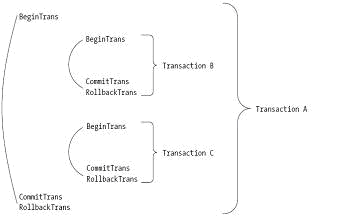
\includegraphics[scale=0.6]{img/TrxOperaciones.png}
		\label{fig:TrxOperaciones.png}
		\caption{Transacciones anidadas como operaciones}
\end{figure}

\subsubsection{Savepoints}

Un savepoint permite establecer un punto significativo dentro de una transacci�n y permite deshacer los cambios hechos desde ese punto en adelante (siempre y cuando no se haya terminado la misma). El uso de estos savepoints est� expuesto a la interfaz de usuario en forma de sentencias como se muestran en el apartado del analizador.\\

Para el usuario, los savepoints toman nombres amistosos. Luego estos se asocian con el ultimo LSN (evento de log, ver apartado de ARIES) de la transacci�n en curso. Si establece un savepoint con un nombre ya tomado, el anterior es borrado. Entre distintas transacciones puede haber savepoints de igual nombre. Esto incluye transacciones anidadas, pues no se puede volver a un savepoint de una transacci�n padre (No se encuentra soportado).\\

%trxSavePoints

\begin{figure}[h]
		\centering
		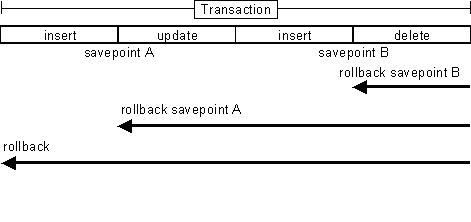
\includegraphics[scale=0.6]{img/trxSavePoints.png}
		\label{fig:trxSavePoints.png}
		\caption{Uso de savepoints}
\end{figure}

Aprovechando la capacidad de savepoints, cuando se ejecutan sentencias dentro de una transacci�n expl�cita, antes de cada una se marca un savepoint de manera autom�tica, as� si ocurre una excepci�n en la ejecuci�n de la misma, se realiza un rollback hasta ese savepoint. Esto excluye excepciones por dead lock, pues ah� se abortan todas las transacciones del thread, para liberar los locks que tuvieran tomados.\\



\subsection{Index Manager}

Este modulo fue creado en vistas de mejorar la concurrencia entre tran-sacciones as� como la performance de las sentencias que consultan las tablas.\\

La finalidad es que cuando se realice una consulta con una expresi�n donde se iguale una columna con un valor, se va a poder usar el �ndice correspondiente de la columna. Luego se van a recorrer los registros de la tabla que existan en ese �ndice, evitando la necesidad de recorrer todos los registros, y poder lograr mayor concurrencia en el caso que hubiera otra transacci�n que realice otra consulta utilizando una expresi�n tal que los registros representados en su �ndice no se encuentren compartidos con la primer transacci�n (ejemplo, una expresi�n donde se iguala la misma columna pero con otro valor tal que su n�mero de hash es distinto).\\

Como los datos de las tablas no se encuentran ordenados, �stos �ndices son del tipo \textit{unclustered}, y como existe una entrada para cada registro de la tabla (seg�n el hash que corresponda), tambi�n son del tipo \textit{densos}.\\

Es necesario mencionar que este motor no tiene implementadas claves primarias ni restricciones de unicidad en las columnas de una tabla. Suelen ser conocidos entonces como �ndices secundarios. En el cap�tulo 8.4 de \cite{RAMA03} se explican y comparan las diferentes propiedades que puede tener un �ndice.\\

Para cada �ndice se utilizan buckets con overflow. (Explicaci�n de �ndices hash con overflow en el cap�tulo 10 de \cite{RAMA03}). Todos los valores posibles de la columna son asignados a un numero hash, y se agrega una entrada en el bucket que corresponda a tal par [columna, hash].
 Al no ser din�mico se puede dar el caso que una entrada de hash tenga muchos buckets, pero aun as� va a ser mas concurrente que recorrer toda la tabla. Adem�s, el objetivo del trabajo pr�ctico es mostrar una implementaci�n y funcionamiento del sistema ARIES. Estos �ndices son solo un agregado para mejorar un poco la concurrencia y proveer nivel aislamiento serializable sin tener que bloquear toda la tabla.\\

El �ndice hash tambi�n es �til para las tablas del catalogo, pues cuando se desea obtener una tabla no es necesario recorrer toda la tabla de tablas busc�ndola.\\

El sistema de ARIES nos va a permitir que los �ndices sean tan transaccionales como las tablas comunes. Se agregaron los eventos (l�gicos) de actualizaci�n de �ndices en el log para realizar REDO y UNDO de los mismos en caso de ser necesario, y se agreg� al sistema de Lock Manager bloqueo sobre los �ndices (ver m�s detalles en la secci�n correspondiente de dicho administrador). Por �ltimo, cuando se modifica alg�n Bucket, de la misma manera que las p�ginas, se toma un Latch para que darle orden a las modificaciones concurrentes.\\

\subsection{Lock Manager}

Este modulo tiene como objetivo administrar los bloqueos tanto de lectura como de escritura. Se utiliza un bloqueo pesimista \cite{RAMA03} en vistas de mostrar su dise�o, implementaci�n y uso de manera educativa, y por ser m�s simple que el mantenimiento de versiones que suelen tener los bloqueos optimistas.\\

En este dise�o se tomo la decisi�n de implementar el protocolo de 2PL, sobre el esquema RLOCK / WLOCK, o sea sobre bloqueos ternarios. En principio se pens� tomando en cuenta las condiciones de los cap�tulos 18 y 19 de \cite{RAMA03}. Tiene soporte para bloqueo de granularidad fina (a nivel de registro) lo que permite una mayor concurrencia entre transacciones.\\

\begin{figure}[h]
		\centering
		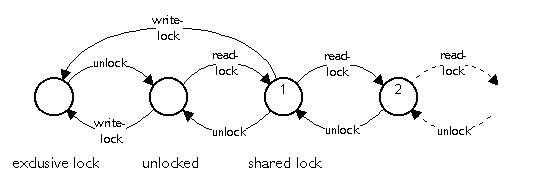
\includegraphics[scale=0.6]{img/LockManager.png}
		\label{fig:LockManager.png}
		\caption{Modelo de Two phase locking}
\end{figure}

Se han implementado los cuatro niveles est�ndar de aislamiento transaccional: READ UNCOMMITTED, READ COMMITTED, REPEATABLE READ y SERIALIZABLE \cite{SQL92}, \cite{RAMA03}. El bloqueo de elementos dentro de una transacci�n se adhiere al protocolo 2PL estricto para los primeros dos niveles \cite{S2PLWIK} y al protocolo 2PL riguroso para los �ltimos dos niveles \cite{R2PLWIK}. Seg�n se muestra en \cite{BERNTS} y en \cite{FRACCR}, se mantiene la correctitud sem�ntica, y los distintos niveles muestran un tradeoff entre performance (menos bloqueos / mayor concurrencia) e inconsistencias posibles en el aislamiento de las transacciones.\\

El Lock Manager est� dise�ado de la siguiente manera:\\

Su estructura cuenta con m�todos para bloquear un elemento (se utiliza el ID del elemento), para desbloquearlo, y para saber si un elemento se encuentra bloqueado.\\

Cuando se desea bloquear un elemento tambi�n se especifica si se desea un bloqueo exclusivo o compartido. En nuestro esquema, el bloqueo exclusivo es utilizado para bloquear objetos para su posterior escritura, y el bloqueo compartido para bloquear elementos que van a ser le�dos.
Estos m�todos se ejecutan de manera sincronizada. Esto es, s�lo una transacci�n (thread/conexi�n) puede estar ejecut�ndolo a la vez. Fue necesario pues las estructuras donde se guardan los Locks son compartidas por todas las conexiones.\\

Al igual que con el resto de los m�dulos relacionados con transacciones, �ste administrador fue luego modificado para dar soporte a transacciones anidadas y Savepoints.\\

Cuando se aborta hasta un Savepoint, se desean liberar aquellos Locks obtenidos luego del mismo. Para ello, se conoce cu�l fue el �ltimo LSN antes de crear un Lock en la transacci�n, y existe un m�todo que libera aquellos Locks mayores al LSN relacionado con el Savepoint.\\

Cuando se crea una transacci�n hija, esta hereda los locks de sus ancestros. Cada Lock guarda qu� transacci�n lo cre�. Pero el algoritmo para saber si un elemento ya se encuentra bloqueado por una transacci�n itera tambi�n por aquellos pertenecientes a transacciones ancestras. Cuando una transacci�n hija es abortada, todos sus locks son liberados de la misma manera que fuera una de nivel alto, pero cuando realiza commit, todos sus locks no son liberados sino delegados a la transacci�n padre. Luego, a medida que vayan haciendo commit se ir�n pasando hasta llegar a la de m�s alto nivel.\\

Un caso especial es cuando una transacci�n ancestra tiene un Lock compartido sobre un elemento, y la descendiente desea actualizar ese Lock a uno exclusivo (para realizar una modificaci�n o borrado del elemento). En este caso ambos Locks se mantienen en las estructuras, para que el bloqueo exclusivo sea liberado en caso de un aborto, o sea delegado al padre en caso de commit. Si el padre era quien pose�a el Lock compartido, el mismo ser� actualizado a exclusivo (como ya hab�a un bloqueo exclusivo, se sabe que ninguna otra transacci�n posee bloqueos compartidos sobre el elemento afectado).\\

\subsubsection{Deadlock}

Para el tratamiento de DeadLocks, se opt� por usar los algoritmos de prevenci�n en vez de detecci�n una vez que ocurrieron. Esto es para mantener la simplicidad del trabajo. Como trabajo futuro se podr�a implementar un algoritmo basado en deadlock detection. Se dise�� una interfaz, la cual es usada por el administrador cada vez que se desea bloquear un elemento, para verificar si puede haber un conflicto entre la transacci�n que desea bloquear con aquellas due�as de Locks sobre el elemento en cuesti�n.\\












\newpage
\section{Implementacion} 

A continuaci�n se describen los temas de implementaci�n, separados por m�dulos para una mejor comprensi�n.\\

\subsection{Plataforma}

El lenguaje elegido para desarrollar el RDBMS fue Java dada la gran cantidad de plugins existentes para hacer interfaces graficas,  as� como la simplicidad de su lenguaje, poder que resulta propicio para la realizaci�n de trabajos acad�micos de este estilo. Utilizamos la versi�n de Java 5.0 que trae mejoras con respecto a las anteriores versiones para simplificar la programaci�n de la aplicaci�n en los aspectos de dise�o y concurrencia. Tambi�n destacamos el haber hecho la implementaci�n usando Patrones de Dise�o, entre los que podemos mencionar: Factory, Strategy, Decorator, Singleton y Abstract factory \cite{GAMMA95}.\\

Entre los plugins utilizados, usamos un CVS remoto para subir las fuentes y ad-ministrar las versiones de los diferentes m�dulos \cite{CVSSSL}. Usamos el Jigloo para crear la interfaz grafica del cliente. \cite{JIGLOO}\\

Para ciertas funcionalidades del sistema utilizamos paquetes especializados, a saber:\\

\begin{itemize}
	\item ZQL: paquete que provee an�lisis de sentencias SQL y la creaci�n de estructuras Java que corresponden a las mismas \cite{ZQL}.\\
	\item SC: librer�a que realiza el coloreo de palabras clave de una sentencia SQL para facilitar la lectura de la misma en el cliente \cite{SYNCOL}.\\

	\item Commons-Collections: conjunto de diferentes estructuras de datos e implementaciones especializadas (Conjunto,  Lista, Mapa) \cite{COMCOL}.\\
\end{itemize}

El sistema sigue el protocolo Cliente - Servidor, en donde el motor de base de datos act�a en un modo pasivo, escuchando por un puerto a que se conecte un cliente. �ste le va haciendo pedidos al servidor, el cual los procesa y devuelve resultados.\\

Ambos programas, al inicializar, abren puertos de escucha utilizando los m�todos provistos por Java y delegando al mismo los detalles de conexi�n.\\
El intercambio de mensajes se hace a trav�s de estos Sockets abiertos, y utilizan un formato de texto simple. Los pedidos del cliente hacia el servidor ser�n las sentencias SQL escritas por el usuario, mientras que los resultados en sentido inverso son los mensajes de respuesta del servidor. 
Esta respuesta puede ser:\\

\begin{itemize}
	\item un mensaje de informaci�n explicando el resultado de la sentencia, cuando esta se ejecuta de manera exitosa. 
\end{itemize}


\begin{itemize}
	\item 	un texto conteniendo los resultados en un formato de tabla cuando la sentencia es una consulta.
\end{itemize}

	
\begin{itemize}
	\item un mensaje con una descripci�n de error cuando ocurre uno al procesar la sentencia.
\end{itemize}

Existen tambi�n dos puertos traseros en el servidor, los cuales sirven para darle informaci�n al cliente administrador sobre el estado de las estructuras de Lock, y de los eventos que van siendo guardados en el Log. �stos son provistos para que los usuarios puedan saber, en tiempo real, los eventos ocurridos dentro del servidor y poder entender los mecanismos del mismo.\\




\subsection{Disk Space Manager}

Cada p�gina ha sido implementada de manera tal que contiene un n�mero fijo de re-gistros, y un n�mero fijo de bytes (64KB). La cantidad de registros depende de las columnas de la tabla, es decir, dependiendo de la cantidad de columnas y tama�o de las mismas. Este formato de p�gina hace que no existan registros guardados en m�s de una p�gina, o sea, cada p�gina guarda una cantidad entera de registros. Esto trae la simplicidad en el motor de transacciones, ya que los eventos de un registro siempre corresponden a una sola p�gina, pero trae la contrariedad de no poder crear tablas cuya longitud de registro sea mayor al tama�o especificado de una p�gina. Esta decisi�n fue tomada con fines de simplificar el motor de transacciones. El tama�o de cada p�gina va a variar dependiendo si se aprovechan los 64KB o, por el hecho de no cortar registros entre 2 p�ginas, si es menor al mismo.\\

La nomenclatura elegida para el nombramiento de los archivos en disco es la siguiente:\\

\begin{itemize}
	\item NumeroTabla.NumeroPagina para identificar un bloque que representa a una p�gina. No se utiliza nombre de tabla porque, como el motor es case sensitive (diferencia los nombres en may�scula y min�scula), esto ocasionaba problemas para quellas plataformas en donde el sistema de archivos I/O es case insensitive.

	\item NumeroTabla.NumeroColumna.NumeroHash.NumeroBucket para los buckets de los �ndices.
\end{itemize}

Las p�ginas guardadas en binario, se mantienen en los slots del Buffer Manager, y son transformadas en objetos entendibles por el motor al momento de la lectura y escritura de registros. Al no haber tipo de datos de longitud variable, revisando en el cat�logo la tabla de columnas es posible saber cu�l es la longitud de cada registro correspondiente a una determinada tabla.\\


Para saber si un registro se encuentra libre u ocupado, se pensaron dos maneras:\\


\begin{enumerate}
	\item guardar al principio de la p�gina un conjunto de bits, en donde si se encuentra encendido el n-�simo bit, quiere decir que el n-�simo registro est� ocupado.
	
	\item que el primer bit de cada registro sea un valor de verdad que indique si el mismo est� libre o no.
\end{enumerate}

La manera (a) tiene la ventaja que es f�cil saber si una p�gina est� vac�a o llena, 
pues todos los bits se encuentran consecutivos y si est�n todos desactivados o activos indican (respectivamente) los estados mencionados. Por otro lado, si en el log de ARIES se guardan los cambios a nivel de bytes, entonces es conveniente que el indicador se encuentre junto con el resto del contenido del registro, como en la manera (b), para guardar en un solo evento los bytes cambiados por la modificaci�n del registro. Como los eventos del log son l�gicos, se decidi� utilizar la opci�n (a). Esta pol�tica est� implementada en la clase ArregloBits.


Adem�s, se crearon m�todos que convierten los elementos Java, que representan los tipos soportados por el motor, a arreglos binarios de tama�o fijo, determinado por el tipo, y que contienen una representaci�n del valor del elemento. Luego se guardan de manera consecutiva estos arreglos de bytes, respetando el orden seg�n las columnas de la tabla. Notar que no se guarda ninguna informaci�n respecto a qu� tipo es o la longitud del arreglo de bytes, pues esta informaci�n se obtiene al consultar los tipos de las columnas de la tabla correspondiente.\\



\subsection{Buffer Manager}

En el momento de realizar el an�lisis previo a la implementaci�n de este proyecto, hemos observado que en la mayor�a de los casos iba a existir una peque�a cantidad de p�ginas con un enorme n�mero de referencias. Por este motivo es que, en nuestro dise�o, decidimos incluir una estructura que nos permita mantener una cierta cantidad de p�ginas en memoria sin la necesidad de leerlas de la memoria secundaria constantemente. Esta estructura encargada de traer p�ginas de memoria secundaria a memoria principal es el Buffer Manager, el cual para este prop�sito, posee una colecci�n de p�ginas llamadas \textbf{Frames} (tambi�n denominadas \textbf{Buffer Pool}). La cantidad de Frames en el pool del Buffer Manager es configurable.\\


\begin{figure}[h]
		\centering
		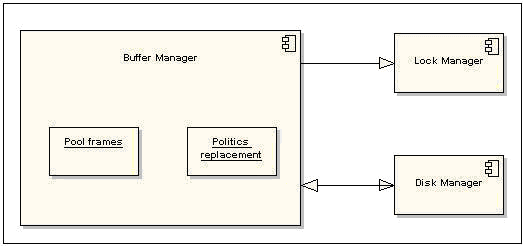
\includegraphics[scale=0.6]{img/BufferManagerImp.png}
		\label{fig:BufferManagerImp.png}
		\caption{Implementaci�n del Buffer Manager de Kanon}
\end{figure}


El pool de Frames est� implementado con un mapa que tiene el ID de una p�gina como clave y la p�gina propiamente dicha como valor. Este mapa se encuentra sincronizado, pues es accedido por varios threads, y sincronizar las operaciones principales del Buffer Manager era demasiado costoso. El tama�o del mapa es configurable, de manera de poder realizar comparaciones entre distintos tama�os para conocer diferencias de performance al utilizar m�s memoria en el pool.\\

Como ya mencionamos, la tarea fundamental del Buffer Manager es traer p�ginas de disco y brindarle a las clases superiores los m�todos necesarios para mantenerlas en memoria hasta que estos digan lo contrario. Sin embargo estas p�ginas liberadas solo ser�n removidas del Buffer y grabadas nuevamente en el disco, en el caso de haber sido modificadas, cuando no existan m�s frames libres en el Buffer y se solicite alocar una p�gina que no se encuentra en el mismo en ese momento.\\

Para realizar este procedimiento utilizamos un algoritmo de remoci�n de p�ginas. La implementaci�n del Buffer Manager utiliza una Interfaz para acceder a la pol�tica de reemplazo. Distintas implementaciones de esta interfaz proveen algoritmos \textbf{FIFO}, \textbf{LRU}, \textbf{MRU}, \textbf{LFU}, \textbf{MFU} y \textbf{remoci�n al azar}. Cada uno de ellos tienes sus ventajas y desventajas seg�n el procedimiento que se est� realizando. Por ello se recomiendan usar h�bridos (por ejemplo, una mezcla entre \textbf{LFU} y \textbf{LRU}). Sin embargo, en vistas de mantener el trabajo simple y entendible, no se han implementado algoritmos avanzados de reemplazo de p�ginas. La pol�tica de reemplazo a utilizar por la aplicaci�n es configurable.\\

Cada p�gina tiene la propiedad de saber si esta sucia o no, es decir, si se modific� desde la �ltima vez que se guard� en disco. Con esta informaci�n, necesaria para el funcionamiento de ARIES, se utiliza la llamada \textbf{Dirty-Pages table}, la cual provee informaci�n sobre las p�ginas que han sido modificadas durante el uso normal de la base de datos. Esta tabla tambi�n es usada cuando se recupera el sistema luego de una ca�da. Cada entrada de la tabla consiste de dos campos: PageID y RecLSN. Durante el procesamiento normal, cuando una p�gina se fija en un slot del Buffer Manager para modificarla, se registra el LSN del pr�ximo evento a ser guardado en el log (o sea, el LSN del fin del log). Este valor indica desde qu� punto en el log pueden haber modificaciones sobre la pagina que probablemente no se encuentren en la versi�n de almacenamiento estable de la misma (�til para saber hasta qu� punto se encontraba actualizada la p�gina en caso de suceder una ca�da). Los contenidos de esta tabla son incluidos en el registro de checkpoint. Luego, cuando se recupera el sistema y se lee dicho registro, se recrea esta tabla  y es modificada durante la fase de An�lisis. El menor valor de RecLSN en la tabla indica el punto de partida para la fase de Redo al momento de recuperar el sistema.\\

Las p�ginas cuentan con una bandera que indica si han sido modificadas. La misma es marcada cuando se realiza una inserci�n, actualizaci�n o remoci�n de un registro de tal p�gina. Luego, antes de remover la p�gina de memoria, el Buffer Manager la persiste (llamando al Disk Space Manager) en caso de estar marcada, para evitar que se pierdan los cambios realizados.\\



\subsection{Ejecutor}

El Server va leyendo cada sentencia que le llega desde el cliente. Por cada una debe: analizarla, ejecutar el comando correspondiente y devolver el resultado o error.\\

Una de las principales caracter�sticas de nuestras clases XQL (las cuales son una translaci�n directa de las clases provistas por el analizador), es que se pueden agregar nuevos componentes f�cilmente sin tener que realizar modificaciones a la clase. Toda clase XQL implementa XStatement con sus 2 m�todos: \texttt{zqlToXql()} y \texttt{execute()}. El primero permite dado un objeto de la clase ZQL (la devuelta por el analizador) copiar y procesar sus componentes a su par en XQL. El m�todo \texttt{execute()} realiza la ejecuci�n propia de cada statement. De esta forma obtenemos un dise�o de c�digo mucho m�s escalable, permitiendo su modificaci�n f�cilmente. Esta implementaci�n es tomada del patr�n de dise�o Strategy \cite{GAMMA95}, cada XQL sabe que hacer, por lo que el ejecutor se desliga de esos detalles.\\

Desde el Servidor, se debe verificar si ya hay una transacci�n abierta o si se debe crear una transacci�n de manera impl�cita para la sentencia que se est� analizando.
Una transacci�n tiene dos formas de iniciarse, de manera expl�cita o impl�cita. De manera expl�cita, el cliente solicita mediante una sentencia (BEGIN TRANSACTION) que desea abrir una transacci�n, y para cerrar la transacci�n el cliente debe indicar si aborta o realiza commit del conjunto de sentencias. De manera impl�cita, el cliente env�a una sentencia sin tener abierta una transacci�n. Para este caso, el servidor inicia una transacci�n para esa sentencia, y una vez ejecutada esa transacci�n procede a realizar commit sin necesidad de confirmaci�n por parte del cliente (en el caso de que se haya lanzado una excepci�n, se aborta la transacci�n).\\

\subsection{Recovery Manager}

Para la implementaci�n orientada a objetos del m�dulo, existen entidades que representan a cada evento posible de los existentes en el log, y a medida que se va leyendo el mismo, estos objetos son creados y dentro de cada uno existe un c�digo propio para las tres fases correspondientes. El prop�sito de la fase de An�lisis es saber cu�les transacciones se encontraban en curso cuando se produjo la ca�da, y que p�ginas conten�an modificaciones que no fueron guardadas en disco. La fase de Redo se encarga de reproducir las modificaciones de todas las transacciones involucradas en aquellas p�ginas no persistidas, y la fase de Undo consiste en luego deshacer los cambios por las transacciones que no hab�an hecho commit. Entonces, los tres ciclos principales en el modulo se encargan de leer el log y crear los eventos, y cada evento sabe qu� hacer seg�n el ciclo que se encuentre. Esto permite una mejor compresi�n del algoritmo de recuperaci�n, as� como tambi�n permite realizar modificaciones al mismo o a eventos en particular sin que ello afecte a las dem�s componentes que interact�an en el proceso.\\

Los eventos disponibles en este proyecto para el modulo de recuperaci�n son:\\

\begin{itemize}
	\item 	Evento de inserci�n de un registro en una p�gina de una tabla: contiene la transacci�n a la que pertenece, el LSN del evento anterior en la transacci�n, el identificador del registro insertado y los valores de cada columna de la tabla afectada.
	
\item Evento de modificaci�n de un registro en una p�gina de una tabla: contiene la transacci�n a la que pertenece, el LSN del evento anterior en la transacci�n, el identificador del registro modificado, los valores originales de las columnas modificadas, y los nuevos valores que ocupar�n las mismas en ese registro.

\item 	Evento de borrado de un registro en una p�gina de una tabla: contiene la transacci�n a la que pertenece, el LSN del evento anterior en la transacci�n, el identificador del registro borrado y los valores originales de las columnas de la tabla para ese registro.

\item 	Evento CLR de inserci�n de un registro en una p�gina de una tabla: contiene la transacci�n a la que pertenece, el LSN del evento anterior en la transacci�n, el identificador del registro insertado y un conjunto de UndoNextLSN (modificaci�n hecha para el soporte de transacciones anidadas, detallada m�s adelante en el texto).

\item 	Evento CLR de modificaci�n de un registro en una p�gina de una tabla: contiene la transacci�n a la que pertenece, el LSN del evento anterior en la transacci�n, el identificador del registro modificado, los valores originales de las columnas afectadas antes por la modificaci�n y un conjunto de UndoNextLSN (modificaci�n hecha para el soporte de transacciones anidadas, detallada m�s adelante en el texto).

\item 	Evento CLR de borrado de un registro en una p�gina de una tabla: contiene la transacci�n a la que pertenece, el LSN del evento anterior en la transacci�n, el identificador del registro borrado, los valores originales de las columnas del registro y un conjunto de UndoNextLSN (modificaci�n hecha para el soporte de transacciones anidadas, detallada m�s adelante en el texto).

\item 	Evento de inserci�n de un registro en una p�gina de un �ndice: contiene la transacci�n a la que pertenece, el LSN del evento anterior en la transacci�n, el identificador del registro-�ndice insertado y el identificador del registro de la tabla referenciado.

\item 	Evento de borrado de un registro en una p�gina de un �ndice: contiene la transacci�n a la que pertenece, el LSN del evento anterior en la transacci�n y el identificador del registro-�ndice borrado.

\item 	Evento CLR de inserci�n de un registro en una p�gina de un �ndice: contiene la transacci�n a la que pertenece, el LSN del evento anterior en la transacci�n, el identificador del registro-�ndice insertado y un conjunto de UndoNextLSN (modificaci�n hecha para el soporte de transacciones anidadas, detallada m�s adelante en el texto).

\item 	Evento CLR de borrado de un registro en una p�gina de un �ndice: contiene la transacci�n a la que pertenece, el LSN del evento anterior en la transacci�n, el identificador del registro-�ndice borrado, el registro de la tabla al cual referenciaba  y un conjunto de UndoNextLSN (modificaci�n hecha para el soporte de transacciones anidadas, detallada m�s adelante en el texto).

\item 	Evento de commit de una transacci�n: contiene la transacci�n a la que pertenece, el LSN del evento anterior en la transacci�n y un conjunto con los identificadores de los registros bloqueados al momento del commit.

\item 	Evento de rollback de una transacci�n: contiene la transacci�n a la que pertenece y el LSN del evento anterior en la transacci�n.

\item 	Evento de fin de una transacci�n: contiene la transacci�n a la que pertenece y el LSN del evento anterior en la transacci�n.

\item 	Evento de Begin Checkpoint: no contiene ning�n par�metro. Es el evento referenciado por el registro maestro al realizarse un Checkpoint, y a partir del cual se empezar� a leer el log cuando se inicia el sistema.

\item 	Evento de End Checkpoint: contiene una lista con las transacciones en curso al momento del Checkpoint. Para cada transacci�n se toma su identificador, �ltimo LSN, estado, conjunto de UndoNextLSN y registros bloqueados al momento de la colecta. Tambien contiene una lista con las p�ginas que no fue
ron persistidas. Para cada p�gina se toma su identificador y LSN del �ltimo evento que la modific�.

\end{itemize}

Las modificaciones de transacciones anidadas mantienen el esquema orientado a objetos ya dise�ado. Se agrega el evento que vincula al commit de una transacci�n hija con la  transacci�n padre, para que en el caso de tener que realizar un Redo o Undo de la �ltima, tambi�n se lo haga de la primera. Este evento se llama CHILD-COMMITTED, toma el identificador de la transacci�n hija y el �ltimo LSN de la misma, y es insertado como un evento de la transacci�n padre. Tambi�n se realizan los cambios mencionados en el algoritmo para que una transacci�n no tenga un solo UndoNextLSN sino un conjunto de ellos durante el aborto, y se ir� tomando el de mayor LSN para seguir un orden cronol�gico inverso.\\

Para agregar el soporte de Nested Top Actions, se agreg� el evento sugerido de DUMMY-CLR. Cuando se comienza con una NTA dentro de una transacci�n, se toma nota del �ltimo LSN de la misma, y luego al finalizar, se escribe el evento DUMMY-CLR. �ste referencia a la LSN mencionada, para que si la transacci�n es deshecha, los eventos correspondientes a la NTA sean salteados (y no deshechos).\\ 


\subsection{Transaction Manager}

El Transaction Manager cuenta con dos mapas de transacciones. Uno asocia cada transacci�n con su identificador, para poder obtenerlas r�pidamente a partir del mismo.
El segundo mapa asocia cada thread con las transacciones en curso. Como se mencion� anteriormente, una lista es usada para las tomar nota de las transacciones anidadas que pueda haber.\\

Existen m�todos para consultar si hay una transacci�n en curso para un thread en particular (sin par�metros asume que se pregunta por el thread que ejecuto el m�todo), para iniciar una transacci�n en un thread, para abortarla (tanto los dos m�todos de aborto mencionados anteriormente, como un m�todo para abortar una transacci�n hasta un savepoint dentro de la misma) o realizar commit.
Para el inicio o fin de cada transacci�n, el transaction manager se comunica con el lock manager para libere los locks correspondientes (si es necesario) y con el Recovery Manager para que se escriban los eventos de fin de transacci�n en el mismo.\\

La profundidad de las transacciones anidadas solo est� limitada por la memoria del sistema.\\

Estructura de una Transacci�n:\\

\begin{itemize}
	\item	Su identificador �nico: para asignarle un id �nico a cada transacci�n se utiliza un numero que va creciendo monot�nicamente.

\item El estado de la misma (en curso, abortada o terminada).

\item	El thread donde se ejecuta la transacci�n.

\item	Un campo timestamp de inicio que marca el momento en el cual empez� la transacci�n, usado para los algoritmos de Prevenci�n de DeadLock.

\item	El LSN del �ltimo evento guardado en el log correspondiente a la transacci�n.

\item	El conjunto de UndoNextLSN. Complementando lo dicho en la bibliograf�a de ARIES con el soporte para transacciones anidadas, el Undo Next LSN es el LSN del pr�ximo evento a ser le�do durante el rollback de la transacci�n. Si durante el rollback se incluyen transacciones hijas de �sta, sus respectivos Undo Next LSN se ir�n guardando en este conjunto, y para el pr�ximo evento a abortar, se elige el de mayor n�mero.

\item	La transacci�n padre de esta, en caso de haber una.

\end{itemize}

\subsection{Index Manager}

Se crea un �ndice para cada columna de cada tabla. No existen las sentencias DDL de manejo de �ndices (CREATE INDEX, DROP INDEX, etc.)\\

Se usa el �ndice correspondiente al primer elemento del WHERE que sea una igualdad. Para mayor informaci�n, consultar la API correspondiente a la ejecuci�n de sentencias que contienen consultas (SELECT, UPDATE Y DELETE). Se recorren solo los registros obtenidos por el �ndice asociado, o todos los registros de la tabla en caso de no poder usar ning�n �ndice.
Formato de un bucket: una lista con los ID de los registros cuyo valor en la columna especificada concuerda con el hash del bucket.\\

 Hay un arreglo de bits que indican los lugares de la lista libres (pueden quedar huecos en el medio de la lista, pero nos evitamos reordenar y el iterador va a ser inteligente y saltea los huecos)
 Cuando se llena un bucket se crea otro (de la misma manera que una p�gina).\\
 
El iterador que devuelva el �ndice va a ser de aquellos registros cuyo valor de hash en la columna concuerde con el hash del valor especificado. O sea, Si pido aquellos registros cuya columna 1 sea igual a "valor1" y "valor2" tiene el mismo hash que "valor1" entonces los �ndices me van a dar no solo aquellos registros cuyo valor en la columna sea "valor1" sino tambi�n los que tienen "valor2". Una optimizaci�n podr�a ser guardar el valor propio en el Bucket, eso har�a que solo se devuelvan los registros de valor "valor1" y aumentar�a la concurrencia.\\

El numero de hash va a ser modulo 8 para evitar que haya muchos buckets con un solo elemento.\\


\subsection{Lock Manager}

En la implementaci�n del Lock Manager se usaron 3 estructuras de datos:\\

Un mapa con ID de clave y un conjunto de Locks por valor:\\

Este mapa permite saber qu� Locks existen actualmente para un elemento dado (especificado seg�n el ID). Pueden existir varios locks compartidos para un elemento, pero si existe un bloqueo exclusivo, va a ser �nico en el conjunto, salvo que haya locks compartidos pertenecientes a transacciones ancestras de aquella que tiene el bloqueo exclusivo.\\
 
Un mapa con ID de clave y una cola de pedidos como valor:\\

Este mapa guarda las transacciones encoladas (usando un orden FIFO) que desean adquirir un Lock para un elemento dado (especificado seg�n el ID). De esta manera se evita inanici�n al querer bloquear un objeto.\\

La estructura de un pedido de bloqueo que se encola contiene los siguientes datos:\\

\begin{itemize}
	\item La transacci�n que realiza el pedido.
\end{itemize}

\begin{itemize}
	\item El thread perteneciente a esa transacci�n ( y que ser� suspendido mientras no se consiga bloquear el objeto)
\end{itemize}

\begin{itemize}
	\item Valor que indica si el bloqueo deseado es exclusivo o compartido.
\end{itemize}

Un mapa por cada Transacci�n con ID de clave y Lock como Valor:\\

Este mapa guarda los Locks adquiridos por cada transacci�n. Es usado para obtener un acceso m�s r�pido a los Locks de la misma, y para mantener la consistencia del sistema de bloqueos.
Cuando se desea bloquear un objeto puede ocurrir que:\\

\begin{enumerate}
	\item	No se encuentre bloqueado: En este caso, se procede al bloqueo efectivo del elemento. En caso de haberse realizado un bloqueo compartido, el administrador comprueba si la cola de conexiones en espera para bloquear el mismo elemento no est� vac�a, y en ese caso de toma la primer conexi�n en espera y le avisa que proceda con su bloqueo (el cual va a ser exitoso en caso de ser un bloqueo compartido y va a volver a esperar en caso de ser uno exclusivo).
	
\item Se encuentre ya bloqueado por la misma conexi�n (ya sea de la misma transacci�n o de alguna ancestra): El bloqueo se deja tal cual estaba, salvo el caso que hubiera un bloqueo compartido y ahora se desee uno exclusivo. Entonces se proceder� a hacer una actualizaci�n del Lock, pero s�lo despu�s de que otras conexiones que tambi�n tuvieran bloqueos compartidos sobre el mismo objeto los hayan liberado.
		
\item Se encuentra ya bloqueado por otra transacci�n (una o varias): Aqu� de nuevo se divide en casos si se desea un bloqueo compartido o exclusivo.

	\begin{enumerate}
	\item  Si se desea un bloqueo compartido y los bloqueos existentes tambi�n son compartidos:
	Si no existe ning�n pedido de bloqueo exclusivo encolado, entonces se realiza el bloqueo y se 			agrega al conjunto de Locks de ese ID. Si existe alguno, �ste pedido se encola al final, esto es 		para que el pedido de bloqueo exclusivo que se encuentra encolado no sufra de inanici�n.


	 \item Si el bloqueo existente es exclusivo, se suspende la transacci�n hasta que tal bloqueo sea 					liberado. Cabe notar que por la cola FIFO, no va a llegar ning�n pedido de bloqueo en el 						 medio, salvo que el mismo sea una actualizaci�n de alg�n bloqueo existente compartido al 					 modo exclusivo.


		\item  Si se desea un bloqueo exclusivo, entonces se encola el pedido. Se espera hasta que todos 			los 	Locks sobre el elemento sean liberados, as� como que ocurran todos los bloqueos encolados 		con	anterioridad.

	\end{enumerate}


\end{enumerate}


Al desbloquear un objeto, si lo que se ten�a sobre tal objeto era un bloqueo exclusivo (se consulta el mapa local para cada conexi�n para averiguar cu�l era el Lock sobre el objeto), entonces luego de desbloquearlo se consulta la cola de espera de tal elemento para que la siguiente conexi�n proceda a la adquisici�n del Lock sobre el objeto.\\

Si se intenta desbloquear un elemento no bloqueado por la conexi�n, se lanzar� una excepci�n.
Para poner en espera a las conexiones que desean adquirir un bloqueo sobre un elemento ya bloqueado, se utilizan los m�todos de suspensi�n de Threads provistos por Java 1.5.\\

Tambi�n se ha implementado un decorador (Del patr�n de dise�o Decorator \cite{GAMMA95} del administrador el cu�l guarda en un registro cada vez que se desea bloquear o desbloquear un elemento. Este registro luego sirve para mostrar como queda el Historial de eventos de bloqueo durante un determinado tiempo.\\
 
Cuando se le pide una tabla al Cat�logo, �ste la decora con una implementaci�n que realiza el bloqueo y desbloqueo de elementos de manera autom�tica, evitando agregar esta complejidad al ejecutor. Antes de ejecutar las operaciones de inserci�n, actualizaci�n y eliminaci�n, se bloquea el elemento a modificar de manera exclusiva, y si no existe ninguna transacci�n en curso, se desbloquea luego de la operaci�n.\\
 
En caso de haber una transacci�n activa, los bloqueos y desbloqueos se realizaran seg�n el nivel de aislamiento correspondiente:\\

\begin{itemize}
	\item READ UNCOMMITTED: No se realiza un bloqueo compartido antes de realizar una lectura. Se realizan bloqueos exclusivos antes de modificaciones o inserciones. Estos bloqueos son liberados cuando se termina la transacci�n (o delegado a la transacci�n padre si existe).

	\item READ COMMITTED: Se realizan bloqueos compartidos antes de realizar lecturas. Estos son liberados inmediatamente luego de la misma. Se realizan bloqueos exclusivos antes de modificaciones o inserciones. Estos bloqueos son liberados cuando se termina la transacci�n (o delegado a la transacci�n padre si existe).
\end{itemize}

\begin{itemize}
	\item REPEATABLE READ: Se realizan bloqueos compartidos antes de realizar lecturas y exclusivos antes de modificaciones o inserciones. Todos los bloqueos son liberados cuando se termina la transacci�n (o delegado a la transacci�n padre si existe).
\end{itemize}

\begin{itemize}
	\item SERIALIZABLE: �dem anterior, pero adem�s, en una lectura se bloquea el �ndice correspondiente o toda la tabla en caso de no utilizarse ninguno, para evitar ``lecturas fantasmas''. 
\end{itemize}

En todos los niveles, al realizar inserciones se bloquean todos los �ndices de las columnas de la tabla (o en caso de modificaciones, los �ndices afectados), para que las lecturas de nivel SERIALIZABLE sepan sobre estas modificaciones o inserciones y se eviten las mencionadas ``lecturas fantasmas''.\\

Se han implementado distintos algoritmos de prevenci�n, como ser Wound - Wait, Wait - Die, Caution Waiting, y una implementaci�n simple que indica que nunca ocurre DeadLock. Al levantar el servidor se puede elegir qu� algoritmo ser� utilizado. Por omisi�n se toma Caution Waiting.\\

Algunas de estas implementaciones utilizan la fecha de comienzo de las distintas transacciones involucradas para decidir cu�l va a ser la v�ctima.\\

\subsubsection{Deadlock}

Para el tratamiento de DeadLocks, se opt� por usar los algoritmos de prevenci�n en vez de detecci�n una vez que ocurrieron. Esto es para mantener la simplicidad del trabajo. Como trabajo futuro se podr�a implementar un algoritmo basado en deadlock detection. Se dise�� una interfaz, la cual es usada por el administrador cada vez que se desea bloquear un elemento, para verificar si puede haber un conflicto entre la transacci�n que desea bloquear con aquellas due�as de Locks sobre el elemento en cuesti�n.


\newpage
\section{Pruebas sobre el sistema}

El objetivo de las pruebas fue principalmente verificar la correctitud
en toda la funcionalidad soportada por el servidor y el cliente.\\

A continuaci�n, ponemos en detalle una de la pruebas realizadas para
observar como se va modificando el log a medida que se ejecutan las
sentencias.\\

\subsection{Pruebas de funcionamiento}

\textbf{Prueba de inserci�n:}

La siguiente prueba muestra el resultado de ejecutar un insert sobre una
tabla existente:\\

\texttt{insert into proveedores values('Sancor', 'Cordoba 5400', 46532456);}\\

El Log registra los siguientes cambios:\\
   \begin{tabular}{|l|l|l|l|l|}
        \hline
         3976&INSERT&IdTx: 4&PrevLSN:0&\\
        \hline
				 &proveedores&Pag: 0&Reg: 0&\\
        \hline
         &&Col: 0&&Sancor\\
        \hline
  			 &&Col: 1&&Cordoba 5400\\
        \hline
  			 &&Col: 2&&46532456\\
        \hline
         4472&PREPARE&IdTx: 4&PrevLSN:4356&\\
        \hline
         &Lock:&proveedores&Pag: 0&Reg: 0\\
        \hline
         4540&END&IdTx: 4&PrevLSN:4472&\\
        \hline
    \end{tabular}\\

El primer evento corresponde a la inserci�n de un registro a la tabla
proveedores de la transacci�n 4, con LSN 3976 crea el registro 0 en la
pagina 0. Tambi�n se muestra en el log el contenido en cada columna.\\

Luego se hace un insert de registros de �ndices por cada columna, los
cuales no se visualizan en el log. Por eso el LSN 4472 tiene
PrevLSN:4356 y no 3976.\\

El evento PREPARE, indica el commit de la transacci�n y muestra los
locks obtenidos por la misma.\\

El evento END, muestra el cierre de la transacci�n.\\

El resultado de ejecutar un select sobre la tabla proveedores muestra lo
siguiente:\\

    \begin{tabular}{|l|c|l|}
        \hline
        \textbf{nombre} & \textbf{direccion} & \textbf{telefono} \\
        \hline
        Sancor&Cordoba 5400&46532456\\
        \hline
    \end{tabular}\\

\textbf{Prueba de rollback:}

Muestra el resultado de ejecutar una transacci�n explicita en la cual
se realiza la inserci�n de dos registros sobre la tabla proveedores y
luego se hace un rollback.\\
\texttt{begin transaction;\\
insert into proveedores values('Parmalat', 'Corrientes 2400',
46843221);\\
insert into proveedores values('La Serenisima', 'Callao 1030',
44327000);\\
rollback transaction;\\}

El log registra los siguientes cambios:\\
   \begin{tabular}{|l|l|l|l|l|}
        \hline
         4604&INSERT&IdTx: 6&PrevLSN:0&\\
        \hline
				 &proveedores&Pag: 0&Reg: 1&\\
        \hline
         &&Col: 0&&Parmalat\\
        \hline
  			 &&Col: 1&&Corrientes 2400\\
        \hline
  			 &&Col: 2&&46843221\\
        \hline
         5100&INSERT&IdTx: 6&PrevLSN:4984&\\
        \hline
         &proveedores&Pag: 0&Reg: 2&\\
        \hline
         &&Col: 0&&La Serenisima\\
        \hline
         &&Col: 1&&Callao 1030\\
        \hline
         &&Col: 2&&44327000\\
        \hline
         5596&ROLLBACK&IdTx: 6&PrevLSN:5480&\\
        \hline
         Lectura: 5596&ROLLBACK&proxLSN:5616&&\\
        \hline
         Lectura: 5480&INSERT\_INDEX&proxLSN:5596&&\\
        \hline
         Lectura: 5364&INSERT\_INDEX&proxLSN:5480&&\\
        \hline
         Lectura: 5248&INSERT\_INDEX&proxLSN:5364&&\\
        \hline
         Lectura: 5100&INSERT&proxLSN:5248&&\\
        \hline
         5868&CLR\_INSERT&IdTx: 6&PrevLSN:5784&\\
        \hline
         &&4984&&\\
        \hline
         &proveedores&Pag: 0&Reg: 2&\\
        \hline
         Lectura: 4984&INSERT\_INDEX&proxLSN:5100&&\\
        \hline
         Lectura: 4868&INSERT\_INDEX&proxLSN:4984&&\\
        \hline
         Lectura: 4752&INSERT\_INDEX&proxLSN:4868&&\\
        \hline
         Lectura: 4604&INSERT&proxLSN:4752&&\\
        \hline
         6196&CLR\_INSERT&IdTx: 6&PrevLSN:6112&\\
        \hline
         &&0&&\\
        \hline
         &proveedores&Pag: 0&Reg: 1&\\
        \hline
         6272&END&IdTx: 6&PrevLSN:6196&\\
        \hline
    \end{tabular}\\

La operaci�n begin inicializa el PrevLSN en 0. Los dos primeros
eventos corresponden a la inserci�n de dos registros en la tabla
proveedores.Luego se muestra el evento de ROLLBACK de la transacci�n 6
y se empieza a recorrer la misma leyendo el log desde la �ltima
operaci�n hasta la primera (aqu� se muestra los eventos sobre los
�ndices).\\

Para cada inserci�n abortada se escribe en el log el evento
CLR\_INSERT (seg�n lo especificado por ARIES). Este muestra la
transacci�n a la que pertenece, los UndoNextLSN, y al final el
registro que se esta removiendo. Los eventos CLR\_INSERT\_INDEX no son
mostrados en la pantalla del log, para mejor lectura.\\

Y por �ltimo se muestra el evento END de finalizaci�n de la
transacci�n 6.\\



\newpage
\section{Conclusiones}

Entre las cosas m�s destacables de haber realizado este trabajo fue la gran cantidad de cosas que pudimos aprender durante el transcurso del proyecto sobre lo que es un RDBMS y los aspectos relacionados con la recuperaci�n a un estado consistente luego de una ca�da.\\

Llegamos a la conclusi�n de que la familia de algoritmos de ARIES para la recuperaci�n y bloqueo es un m�todo muy ingenioso y eficaz que es muy usado actualmente en la industria por muchos de los motores relacionales de uso comercial y tambi�n otros para uso acad�mico. Este m�todo encara con precisi�n todos los problemas reales de concurrencia y recuperaci�n que est�n presentes en los RDBMS actuales que se usan �mbitos industriales.\\

Aprendimos de un sistema como ARIES, lo implementamos y nos dimos cuenta del buen funcionamiento y que tan complejo puede llegar a ser el manejo de los problemas de concurrencia y recuperaci�n. En un principio cre�mos que este m�todo s�lo era de aplicaci�n acad�mica pero luego vimos que era ampliamente utilizado y en varios casos extendido o personalizado de maneras interesantes (como paralelizaci�n de la recuperaci�n o uso de versionado en las p�ginas).\\

Este trabajo va servir de ayuda para comprender y observar el funcionamiento de un RDBMS ya que fue pensado con fines acad�micos reflejando de la forma m�s sencilla posible el funcionamiento interno del motor hacia el usuario. Mostramos como se implementa, desde cero, ARIES con un modelo acad�mico simple, modular, orientado a objetos, donde quien est� interesado en el tema puede ver el funcionamiento de ARIES en su totalidad para una mayor comprensi�n.\\

La metodolog�a que plantea el paper de ARIES se acopla bien con temas complejos como anidamiento de transacciones, recuperaci�n de ca�das o savepoints.\\








\newpage
\section{Trabajo futuro}

En este trabajo construimos un motor de base de datos relacional con prop�sitos acad�micos
Que utiliza el m�todo de ARIES para el manejo de transacciones y el aspecto de la recuperaci�n ante ca�das imprevistas del sistema.\\

Esta implementaci�n no contempla algunas temas que son muy interesantes en la actualidad como las transacciones distribuidas y transacciones de larga duraci�n; cuestiones abiertas y de investigaci�n en muchas universidades.\\

Una de las principales ideas a futuro es extender este trabajo implementando una versi�n distribuida de ARIES ( como por ejemplo, D-ARIES ) y que preserve todas las ventajas de ARIES como partial rollbacks , repeatable history, etc.\\

Otro aspecto a mejorar podr�a ser la etapa de An�lisis que se hace durante la recuperaci�n. El cambio consistir�a en paralelizar algunas de las etapas de recuperaci�n de ARIES para ganar eficiencia, otra forma de optimizar ser�a hacer que en la etapa de Redo, �stos sean selectivos, es decir evitar rehacer transacciones que luego se van a deshacer en la etapa de Undo. De esta manera se lograr�a ganar eficiencia en la parte de recuperaci�n.\\

Mientras se hacen las fases de recuperaci�n, que vaya escuchando nuevos pedidos para que sea m�s eficiente el arranque.\\

Soportar media recovery (soporte para copias de seguridad y recupera-ci�n frente a errores ocurridos si se rompe el disco).\\

Deadlock detection en vez de deadlock prevention. Detalles sobre deadlock prevention se pueden encontrar en la secci�n 19.2.2 de \cite{RAMA03}.\\

Agregar un conector est�ndar JDBC (acceder a la DBMS con un cliente JDBC).\\

Mejorar el sistema de �ndices en base a la mejoras descrip-tas en \cite{ARIESIM}, \cite{ARIESKVL} y \cite{ARIESLHS}.\\

Agregar soporte para suspender una transacci�n y luego reanudarla y seguir ejecut�ndola.\\

   


\newpage
\begin{thebibliography}{99}

 \bibitem[ALTIBAS]{ALTIBAS} Jung, Kwang-Chul - Lee, Kyu-Woong \emph{Implementing Storage Manager in Main Memory DBMS ALTIBASE}

 \bibitem[ARIES]{ARIES} Mohan, C. et al \emph{ARIES: A Transaction Recovery Method Supporting Fine-Granularity Locking and Partial Rollbacks Using Write-Ahead Logging}

 \bibitem[ARIESIM]{ARIESIM} Mohan, C. - Levine, F. \emph{ARIES/IM: An Efficient and
High Concurrency Index Management Method Using Write-Ahead Logging}

 \bibitem[ARIESKVL]{ARIESKVL} Mohan, C. \emph{ARIES/KVL A Key-Value Locking Method for Concurrency Control of Multiaction Transactions Operating on B-Tree Indexes}

 \bibitem[ARIESLHS]{ARIESLHS} Mohan, C. - Rothernlel, K. \emph{ARIES/LHS: A Concurrency Control and
Recovery Method Using Write-Ahead Logging for Linear Hashing with Separators}

 \bibitem[ARIESNT]{ARIESNT} Mohan, C. - Rothernlel, K. \emph{ARIES/NT: A Recovery Method Based on Write-Ahead Logging for Nested Transactions}

 \bibitem[ARIESRH]{ARIESRH} Mohan, C. \emph{Repeating History Beyond ARIES}

 \bibitem[BDFCEN]{BDFCEN} Fundamentals of Databases Course \\ \emph{http://www-2.dc.uba.ar/materias/bd}

 \bibitem[BERNTS]{BERNTS} Bernstein, Arthur J. et al \emph{Using Transaction Semantics to Increase Performance}

 \bibitem[BERN87]{BERN87} Bernstein, P. - Hadzilacos, V. - Goodman, N. \emph{Concurrency Control and Recovery in Database Systems, Addison Wesley. 1987}

 \bibitem[BRUNI02]{BRUNI02} Bruni, P. et al \emph{Application Recovery Tool for IMS and DB2 Databases
A Data Recovery Guide}
 
 \bibitem[COMCOL]{COMCOL} Jakarta Commons Collections Homepage\\    \emph{http://jakarta.apache.org/commons/collections/}

 \bibitem[CVSSSL]{CVSSSL} An SSL connection method for CVS (sserver) \\  \emph{http://home.arcor.de/rolf\_wilms/cvsssl/cvsssl\_help.html}

 \bibitem[DCFCEN]{DCFCEN} Computer Science Department \\ \emph{http://www.dc.uba.ar}

 \bibitem[DERBY]{DERBY} DERBY Homepage \\ \emph{http://db.apache.org/derby/papers/recovery.html}

 \bibitem[FCEN]{FCEN} Facultad de Ciencias Exactas y Naturales \\ \emph{http://www.fcen.uba.ar}

 \bibitem[FRACCR]{FRACCR} Franklin, Michael J. \emph{Concurrency Control and Recovery}

 \bibitem[GAMMA95]{GAMMA95} Gamma, E. et al \emph{Design Patterns, Elements of Reusable Object-Oriented Software}

 \bibitem[GRAY80]{GRAY80} Gray, J. et al \emph{The Recovery Manager of the System R Database Manager}

 \bibitem[JIGLOO]{JIGLOO} JIGLOO Homepage \emph{http://www.cloudgarden.com/jigloo/}
 
 \bibitem[KANONOP]{KANONOP} Leggieri, L. - Berlin, J. - Cabas, V. - Pippia, F. \\ \emph{KANON dbms Operations manual}

 \bibitem[KB230785]{KB230785} Microsoft Knowledge Base \\ \emph{http://support.microsoft.com/kb/q230785}

 \bibitem[LEAP]{LEAP} LEAP Homepage \emph{http://leap.sourceforge.net/}
  
 \bibitem[MINIBAS]{MINIBAS} MiniBase Homepage \\ \emph{http://www.cs.wisc.edu/coral/mini\_doc/project.html} 
 
 \bibitem[MINIREL]{MINIREL} Minirel Homepage \\  \emph{http://www.ceid.upatras.gr/courses/minibase/minibase-1.0/documentation/html/minibase/logMgr/report/main.html} 

 \bibitem[ORACLE]{ORACLE} Oracle technology network \\
 \emph{http://www.oracle.com/technology/deploy/availability/htdocs/\\Flashback\_Overview.htm}

 \bibitem[RAMA03]{RAMA03} Ramakrishnan, R. - Gherke, J. \emph{Database Management Systems, 3rd Ed. Mc Graw-Hill, 2003}

 \bibitem[R2PLWIK]{R2PLWIK} Rigurous Two-Phase Locking\\ \emph{http://en.wikipedia.org/wiki/Rigorous\_two-phase\_locking}

 \bibitem[SHAWIK]{SHAWIK} Shadow Paging \emph{http://en.wikipedia.org/wiki/Shadow\_paging}

 \bibitem[SQL92]{SQL92} Isolation Levels \\ \emph{http://en.wikipedia.org/wiki/Isolation\_(computer\_science)}

 \bibitem[STONE76]{STONE76} Stonebraker, M. - Wong, E. - Kreps, P. - Held, G. \emph{The Design and Implementation of INGRES, ACM Transactions on Database Systems, 1976}
 
 \bibitem[SYNCOL]{SYNCOL} JAPISOFT JSyntaxColor \\ \emph{http://www.japisoft.com/syntaxcolor/}

 \bibitem[S2PLWIK]{S2PLWIK} Strict Two-Phase Locking\\ \emph{http://en.wikipedia.org/wiki/Strict\_two-phase\_locking}
 
 \bibitem[ULLMAN88]{ULLMAN88} Ullman \emph{Principles of Database and Knowledge Base Systems, Computer Science Press, 1988}

 \bibitem[WALWIK]{WALWIK} Write-Ahead Logging \\ \emph{http://en.wikipedia.org/wiki/Write\_ahead\_logging}
 
 \bibitem[ZQL]{ZQL} ZQL Homepage \emph{www.experlog.com/gibello/zql/}
 
\end{thebibliography}


\end{document}
